\chapter{Cơ sở lý thuyết}
\label{Chapter3}

\emph{Chương này sẽ trình bày, mô tả chi tiết về các nghiên cứu sẽ thực hiện để giải quyết bài toán xây dựng chatbot chỉ đường, bao gồm việc xác định ý định và trích xuất thực thể}

\section{Hiểu ngôn ngữ tự nhiên - \ac{nlu}}

hiểu ngôn ngữ tự nhiên (\ac{nlu}) là một chủ đề của xử lý ngôn ngữ tự nhiên trong lĩnh vực trí tuệ nhân tạo. Đây có thể nói là thành phần quan trong nhất của chatbot. Chatbot có thật sự thông minh hay không thì đây chính là thành phần quyết định. Mục tiêu của thành phần này là phân loại ý định (intent) và trích xuất thực thể (entity).

Bất cứ khi nào người dùng tương tác với \ac{ai} bằng ngôn ngữ tự nhiên, các từ của họ cần phải được dịch thành một mô tả mà máy có thể đọc được về ý của họ.
Công cụ hiểu ngôn ngữ tự nhiên (\ac{nlu}) trước tiên phát hiện ý định của người dùng là gì (intent), sau đó trích xuất các tham số (entity) của truy vấn. Sau đó, nhà phát triển có thể sử dụng điều này để xác định hành động hoặc phản hồi thích hợp.

Các khái niệm cơ bản:
\begin{enumerate}
    \item Xác định ý định (intent) người dùng
          \\
          Thông thường, người dùng thường truy cập hệ thống chatbot với mong muốn hệ thống sẽ đưa ra những hành động trợ giúp mình về một vấn đề nào đó. Ví dụ, người dùng của hệ thống chatbot hỗ trợ đặt vé máy bay có thể đưa ra yêu cầu đặt vé của mình khi bắt đầu cuộc hội thoại. Để đưa ra hỗ trợ được chính xác, chatbot cần xác định được ý định (intent) đó của người dùng. Việc xác định ý định (intent) của người dùng sẽ quyết định hội thoại tiếp theo giữa người và chatbot sẽ diễn ra như thế nào. Vì thế, nếu xác định sai ý định (intent) người dùng, chatbot sẽ đưa ra những phản hồi không đúng, không hợp ngữ cảnh. Khi đó, người dùng có thể thấy chán ghét và không quay lại sử dụng hệ thống. Bài toán xác định ý định (intent) người dùng vì thế đóng vai trò rất quan trọng trong hệ thống chatbot.
          \\
          Đối với miền ứng dụng đóng, chúng ta có thể giới hạn rằng số lượng ý định (intent) của người dùng nằm trong một tập hữu hạn những intent đã được định nghĩa sẵn, có liên quan đến những nghiệp vụ doanh nghiệp mà chatbot có thể hỗ trợ. Với giới hạn này, bài toán xác định ý định (intent) người dùng có thể quy về bài toán phân lớp văn bản. Với đầu vào là một câu giao tiếp của người dùng, hệ thống phân lớp sẽ xác định ý định (intent) tương ứng với câu đó trong tập các ý định (intent) đã được định nghĩa.
    \item Trích xuất thông tin
          \\
          Bên cạnh việc xác định ý định (intent) trong câu hội thoại của người dùng, chúng ta cần trích xuất các thông tin cần thiết trong đó. Các thông tin cần trích xuất trong một câu hội thoại thường là các thực thể (entity) thuộc về một loại nào đó. Ví dụ, khi một khách hàng muốn đặt vé máy bay, hệ thống cần biết địa điểm xuất phát và địa điểm khách muốn đến, ngày giờ khách hàng muốn bay,…Thành phần hiểu ngôn ngữ tự nhiên (\ac{nlu}) của các hệ thống chatbot thường hỗ trợ các loại thực thể sau (tham khảo tài liệu \cite{1}):

          \begin{itemize}
              \item[--] Vị trí (Location)
              \item[--] Thời gian (Datetime)
              \item[--] Số (Number)
              \item[--] Địa chỉ liên lạc (Contact)
              \item[--] Khoảng cách (Distance)
              \item[--] Khoảng thời gian (Duration)
          \end{itemize}
          Đầu vào của một module trích xuất thông tin là một câu hội thoại. Module trích xuất thông tin cần xác định vị trí của các thực thể trong câu (vị trí bắt đầu và vị trí kết thúc của thực thể). Ví dụ sau minh hoạ một câu hội thoại và các thực thể được trích xuất từ đó.
          \\
          Câu hội thoại: Tôi muốn đặt vé máy bay đi Phú Quốc từ sân bay Nội Bài lúc 8 giờ tối ngày mai.
          \\
          Câu có các thực thể được xác định: Tôi muốn đặt vé máy bay đi [Phú Quốc]LOCATION từ sân bay [Nội Bài]LOCATION lúc [8 giờ tối ngày mai]TIME.
          \\
          Trong câu trên có 3 thực thể (nằm trong các dấu [ ]) với các loại thực thể tương ứng.
\end{enumerate}

\section{Xác định ý định (intent)}

Để xây dựng một mô hình phân lớp ý định (intent), chúng ta cần một tập dữ liệu huấn luyện bao gồm các cách diễn đạt khác nhau cho mỗi ý định (intent). Ví dụ, cùng một mục đích hỏi về thời tiết ở Hà Nội trong ngày hôm nay, người dùng có thể dùng những cách diễn đạt sau:

\begin{itemize}
    \item[--] Thời tiết hôm nay ở Hà Nội thế nào ạ?
    \item[--] Hà Nội hôm nay có mưa không vậy?
    \item[--] Hà Nội hôm nay bao nhiêu độ vậy?
    \item[--] Cho mình hỏi, ra ngoài đường hôm nay có phải mang áo mưa không?
\end{itemize}
Có thể nói, bước tạo dữ liệu huấn luyện cho bài toán phân lớp ý định (intent) là một trong những công việc quan trọng nhất khi phát triển hệ thống chatbot và ảnh hưởng lớn tới chất lượng sản phẩm của hệ thống chatbot về sau. Công việc này cũng đòi hỏi thời gian, công sức khá lớn của nhà phát triển chatbot.

\textbf{Mô hình học máy cho bài toán phân lớp ý định (intent) người dùng:}

Khi đã có dữ liệu huấn luyện cho bài toán phân lớp ý định (intent), chúng ta sẽ mô hình bài toán thành bài toán phân lớp văn bản. Bài toán phân lớp văn bản (text categorization) là một bài toán kinh điển trong ngành NLP và khai phá văn bản (Text Mining). Mô hình phân lớp văn bản cho bài toán phân lớp ý định (intent) được phát biểu một cách hình thức như sau:

Chúng ta được cho trước một tập huấn luyện bao gồm các cặp (câu hội thoại, intent), D = {(x(1), y(1)),…, (x(n), y(n))}, trong đó x(i) là các câu hội thoại và y(i) là ý định (intent) tương ứng cho x(i). Các ý định (intent) y(i) nằm trong một tập hữu hạn K các ý định (intent) được định nghĩa trước. Chúng ta cần học từ tập huấn luyện này một mô hình phân lớp, có chức năng phân lớp một câu hội thoại mới vào một trong các ý định (intent) thuộc tập K. Kiến trúc của hệ thống phân lớp ý định (intent) được minh hoạ như hình (Xem hình Kiến trúc của hệ thống phân lớp ý định (intent) \ref{fig:system-class-intent}).
\begin{figure}[htp]
    \centering
    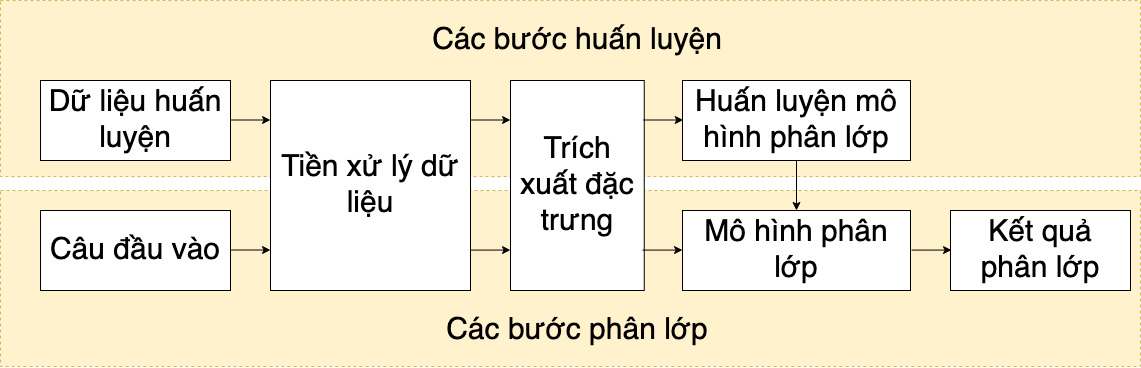
\includegraphics[width=15cm]{images/structure-system-class-intent.png}
    \caption{Kiến trúc của hệ thống phân lớp ý định (intent)}
    \label{fig:system-class-intent}
\end{figure}

Hệ thống phân lớp ý định (intent) có một số thành phần cơ bản:
\begin{itemize}
    \item[--] Tiền xử lý dữ liệu
    \item[--] Trích xuất đặc trưng
    \item[--] Huấn luyện mô hình
    \item[--] Phân lớp
\end{itemize}
Trong bước tiền xử lý dữ liệu, chúng ta sẽ thực hiện các thao tác “làm sạch” dữ liệu như: loại bỏ các thông tin dư thừa, chuẩn hoá dữ liệu như chuyển các từ viết sai chính tả thành đúng chính tả, chuẩn hoá các từ viết tắt,… Việc tiền xử lý dữ liệu có vai trò quan trọng trong hệ thống chatbot do đặc thù của ngôn ngữ chat, nói: viết tắt, sai chính tả, hay dùng “teencode”.

Sau khi tiền xử lý dữ liệu và thu được dữ liệu đã được làm sạch, chúng ta sẽ trích xuất những đặc trưng từ dữ liệu này. Trong học máy, bước này được gọi là trích xuất đặc trưng (feature extraction hay feature engineering). Trong mô hình học máy truyền thống (trước khi mô hình học sâu được áp dụng rộng rãi), bước trích xuất đặc trưng ảnh hưởng lớn đến độ chính xác của mô hình phân lớp. Để trích xuất được những đặc trưng tốt, chúng ta cần phân tích dữ liệu khá tỉ mỉ và cần cả những tri thức chuyên gia trong từng miền ứng dụng cụ thể.

Bước huấn luyện mô hình nhận đầu vào là các đặc trưng đã được trích xuất và áp dụng các thuật toán học máy để học ra một mô hình phân lớp. Các mô hình phân lớp có thể là các luật phân lớp (nếu sử dụng decision tree) hoặc là các vector trọng số tương ứng với các đặc trưng được trích xuất (như trong các mô hình logistic regression, SVM, hay mạng Neural).

Sau khi có một mô hình phân lớp ý định (intent), chúng ta có thể sử dụng nó để phân lớp một câu hội thoại mới. Câu hội thoại này cũng đi qua các bước tiền xử lý và trích xuất đặc trưng, sau đó mô hình phân lớp sẽ xác định “điểm số” cho từng ý định (intent) trong tập các ý định (intent) và đưa ra ý định (intent) có điểm cao nhất.

\section{Trích xuất thông tin}

Cách tiếp cận phổ biến cho bài toán trích xuất thông tin là mô hình hoá bài toán thành bài toán gán nhãn chuỗi (sequence labeling). Đầu vào của bài toán gán nhãn chuỗi là một dãy các từ, và đầu ra là một dãy các nhãn tương ứng các các từ trong đầu vào. Chúng ta sẽ sử dụng các mô hình học máy để học một mô hình gán nhãn từ một tập dữ liệu đầu vào bao gồm các cặp (x1…xn, y1…yn), trong đó x1…xn là dãy các từ, y1…yn là dãy các nhãn. Độ dài của các dãy từ trong tập dữ liệu có thể khác nhau.

Trong bài toán trích xuất thông tin, tập nhãn cho các từ trong câu đầu vào thường được tạo ra theo  mô hình BIO, với B là viết tắt của “Beginning”, I là viết tắt của “Inside”, và O là viết tắt của “Outside”. Khi biết vị trí từ bắt đầu của một thực thể và các từ nằm trong thực thể đó, chúng ta có thể xác định vị trí của thực thể trong câu. Trong ví dụ ở trên, dãy các nhãn tương ứng với dãy của các từ trong câu hội thoại đầu vào được minh hoạ ở bảng \ref{fig:model-BIO}.

\begin{table}[]

\begin{center}
\scalebox{0.5}{
\begin{tabular}{|l|l|l|l|l|l|l|l|l|l|l|l|l|l|l|}
\hline
Tôi & muốn & đặt & vé & máy bay & đi & Phú Quốc   & sân bay & Nội Bài    & vào & 8      & giờ    & tối    & ngày   & mai    \\ \hline
O   & O    & O   & O  & O       & O  & B-LOCATION & O       & B-LOCATION & O   & B-TIME & I-TIME & I-TIME & I-TIME & I-TIME \\ \hline
\end{tabular}}
    \caption{Gán nhãn từ theo mô hình B-I-O trong trích xuất thông tin}
    \label{fig:model-BIO}
    \end{center}
 
\end{table}

Thuật toán huấn luyện mô hình gán nhãn chuỗi phổ biến là mô hình Markov ẩn (HMM – Hidden Markov Models) \cite{2}, mô hình CRF (Conditional Random Fields) \cite{3}. Với dữ liệu văn bản, mô hình CRF thường cho kết quả tốt hơn mô hình HMM. Có khá nhiều các công cụ mã nguồn mở cài đặt mô hình CRF cho bài toán gán nhãn chuỗi như CRF++ \cite{4}, CRF Suite \cite{5}, Mallet \cite{6},…


